\renewcommand{\theequation}{\theenumi}
\begin{enumerate}[label=\arabic*.,ref=\thesubsection.\theenumi]
\numberwithin{equation}{enumi}
\item From the gernelised form of the eqautions 
\begin{align}
minZ &= c^t \vec{x}
\\
\text{subjected to}
\\
A\vec{x} &\preceq b
\\ 
\text{we can find $\to$ }
\\
 c &= \myvec{3 \\ 2}
 \\
 A &= \myvec{-1 & -1 \\ 3 & 5}
 \\
 b &= \myvec{-8 \\ 15}
 \\
 \end{align}\\
  Solution for the above equations can be find from the python code of Lenear programing. 
  \begin{lstlisting}
  ./optimization/codes
  \end{lstlisting}
  From the codes we get that there is no such a point which is common to the both constraints.
  
  \begin{figure}[!ht]
  	\centering
  	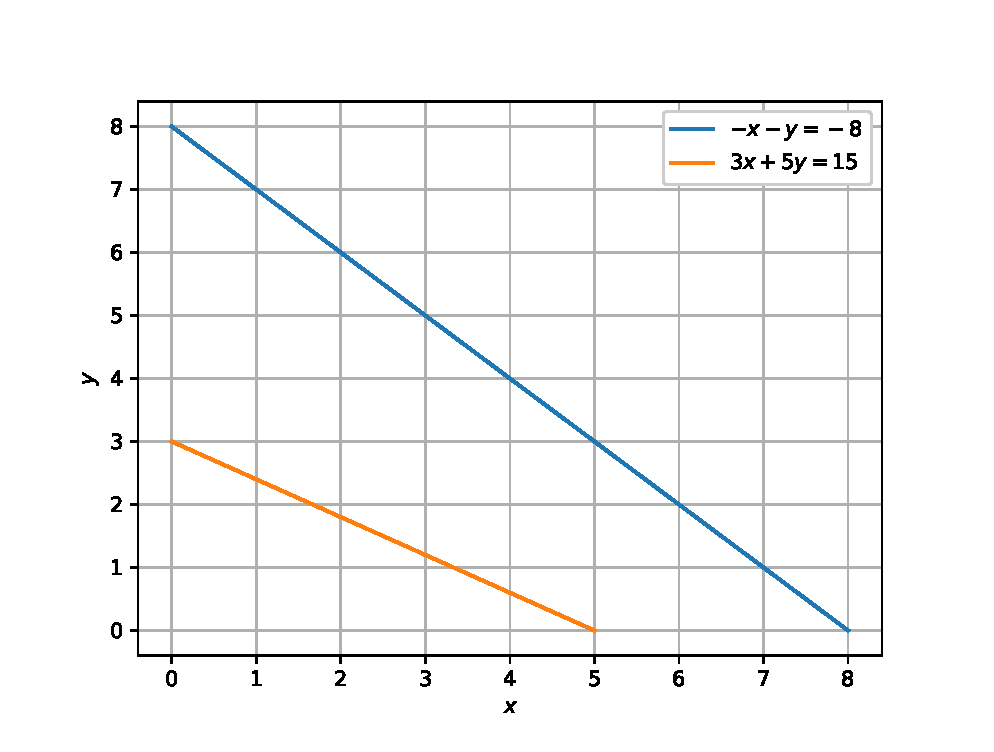
\includegraphics[width=\columnwidth]{./figures/lp1.eps}
  	\caption{ lp1 }
  	\label{fig:lp1}
  Pythone codes for the above figure can be get from
  \begin{lstlisting}
  ./optimization/figures/lp1.eps
  \end{lstlisting}	
  \end{figure}
\end{enumerate}